\documentclass{article}

\usepackage{pgfplots}
\usepackage{amsmath}
\usepackage[margin=1in]{geometry}

\pgfplotsset{compat=1.18}

\begin{document}

\begin{figure}[t]
\centering
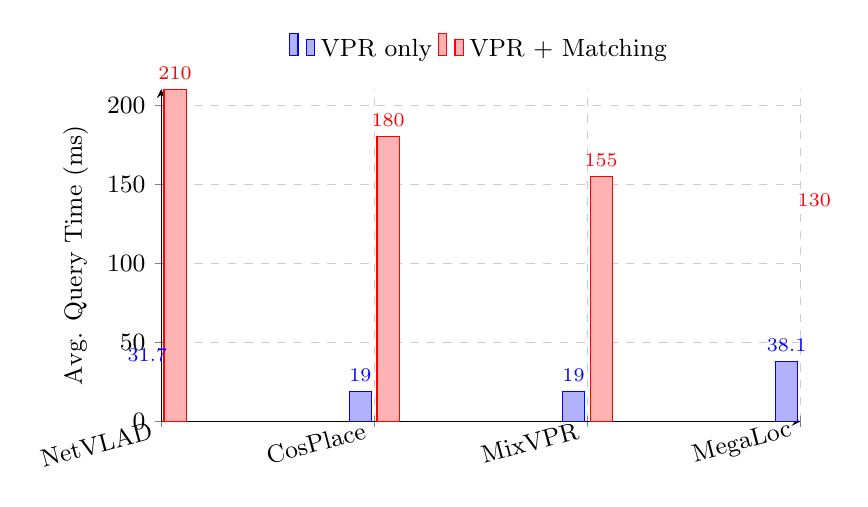
\begin{tikzpicture}
\begin{axis}[
    ybar,
    bar width=8pt,
    width=0.8\textwidth,
    height=5.8cm,
    ymin=0,
    ylabel={Avg. Query Time (ms)},
    symbolic x coords={
        NetVLAD,
        CosPlace,
        MixVPR,
        MegaLoc
    },
    xtick=data,
    xticklabel style={rotate=15, anchor=east},
    tick label style={font=\small},
    label style={font=\small},
    legend style={
        font=\small,
        at={(0.5,1.05)},
        anchor=south,
        legend columns=2,
        draw=none
    },
    nodes near coords,
    nodes near coords style={font=\scriptsize},
    grid=major,
    major grid style={dashed, gray!40},
    axis lines=left
]

% ----------- DATA (replace with real values) -----------
\addplot coordinates {
    (NetVLAD, 31.7)
    (CosPlace, 19.0)
    (MixVPR, 19.0)
    (MegaLoc, 38.1)
};

\addplot coordinates {
    (NetVLAD, 210)
    (CosPlace, 180)
    (MixVPR, 155)
    (MegaLoc, 130)
};
% ------------------------------------------------------

\legend{VPR only, VPR + Matching}

\end{axis}
\end{tikzpicture}
\caption{Average query processing time comparison between VPR-only and VPR with image matching.}
\label{fig:vpr_vs_matching_time}
\end{figure}

\end{document}
